\documentclass[11p]{article}
% Packages
\usepackage{amsmath}
\usepackage{graphicx}
\usepackage[swedish]{babel}
\usepackage[utf8]{inputenc}
\usepackage[T1]{fontenc}

\usepackage[
    backend=biber,
    style=authoryear-ibid,
    sorting=ynt
]{biblatex}
%Källor
\addbibresource{mall.bib}
\graphicspath{ {./images/} }

\title{PMmall \\ \small Fysik 1}
\author{Endo Axelsson}
\date{\today}


\begin{document}

    \begin{titlepage}
        \begin{center}
            \vspace*{1cm}

            \Huge
            \textbf{Vindkraftverk}

            \vspace{0.5cm}
            \LARGE
            El från vinden

            \vspace{1.5cm}

            \textbf{Endo Axelsson}

            \vfill

            Ett PM om vindkraftverk\\
            Fysik 1

            \vspace{0.8cm}

            
\includegraphics[width=0.4\textwidth]{../images/NTI Gymnasiet_Symbol_print_svart.png}

            \Large
            Teknikprogrammet\\
            NTI Gymnasiet\\
            Umeå\\
            \today

        \end{center}
    \end{titlepage}
% Om arbetet är långt har det en innehållsförteckning, annars kan den utelämnas
    \tableofcontents
    \newpage

    \section{Inledning}
    Vi behöver en ny och mer miljövänlig energikälla för jordens hälsa långsiktigt.
    En energikälla som inte är  beroende av olja och brännbara fossiler.
    Detta är ett relevant ämne som diskuteras runtom hela världen för att minska växthus effekten.
    Vilken källa är bäst och hur mycket av det finns det?
    Dem naturliga energikällorna är temat som pratas mycket om och vindkraft är en av dem.
    Men som allt annat så har allt positivt också något negativt och vindkraft är inte ett undantag.
    Så det finns det såklart frågor runtom vindkraften också.
    \subsection{frågeställningar}
    \begin{enumerate}
        \item Vindkraft, så fungerar det
        \item Globala och lokala miljöpåverkan av vindkraft
        \item Vindkraftens påverkan på områden och ekonomi
        \item Vindkraft, land eller vatten?
    \end{enumerate}

    \section{Resultat}

    \subsection{Vindkraft, så fungerar det}

  Vindkraftens funktion är i princip rätt så simpelt, Som namnet utger så kommer energin från vinden.
  Vinden blåser mot vindkraftverken och möter rotorbladen, detta tillför mekanisk energi som får
  bladet att rotera sig.
  Bladet sitter samman med en maskinhus som i sin del genererar elelektrisk
  energi.
  Denna energin åker ner till en transformator där energin justeras så att den kan tillföras
  vidare till hus och andra grejer.

  Det praktiska är att vindriktningen faktist inte spelar någon  roll.
   Alla vindkraftverk som inte är i äldre versioner har turbiner som roterar sig till rätt riktning. (se figur 1)

    \endsubsection

    \begin{figure}
        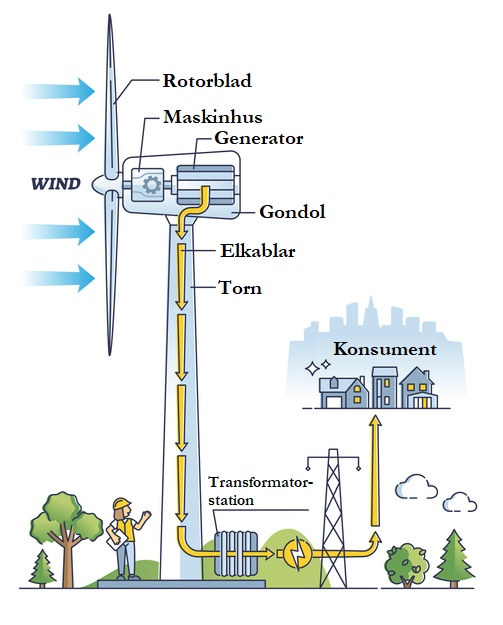
\includegraphics[width=0.6\textwidth]{../images/vindhur.jpg}
        \caption{funktionen simplifierad. Källa: Ugglasno.se}
    \end{figure}

    \subsection{Globala och lokala miljöpåverkan av vindkraft}
    Miljöpåverkan på olika saker är en stor fråga som är aktuellt.
    Fokuset är att hitta en energikälla som inte är begränsad av och påverkar miljön lika mycket som källorna som är vanligast.
    När hela världens länder snackar om energikällor så handlar det ofta om hur den aktiva tillverkningen av energin och produktionen påverkar miljön.
    Själva monteringen och konstrueringen av vindkraftverk är det som kostar som mest och har mest effekt på miljön.
    Men när allt väl är uppe så är vindkraftverk väldigt bra, långsiktigt så är det en stabil källa om man endast tänker på miljö perspektivet.
    Som\parencite{ugglansfysik} tar upp på deras sida.
    Fördelerna är många: för det första så är det lite underhåll, det är ingen restfall efter, de är inte lika stor påverkan på naturlivet runt om, energin är förnybar, gratis och den största fördelen är att den inte bidrar till växthuseffekten ()


    \subsection{Vindkraftens påverkan på samhället och ekonomi}
   I en artikel så nämner \textcite{divaportal} om hur medborgare är oroliga över de sjunkande fastighetspriserna i områderna med vindraftverk runtom.
    Folk som då har vindkraftverk runtom sina bostader tycker att vindkraftverken förstör landskapsbilden.Dem är fula och bullrar.
    Men för dem som inte har dem runtom sig tycker att det är en rätt så bra energikälla, och det blir lite konflikt där.
    På den ekonomiska sidan så kostar vindkraftet inte mycket alls långsiktigt till skillnad till de andra, på grund av de låga underhållningen och tjänst som behövs.
    Tekniken runtom vindkraftverken har utvecklats, och det finns bevis och statistik för det.
    Sidan \textcite{elektrikern} hävdar att priset har gått ner från 45 öre per kilowatt till under 30 öre.
    Och dessutom så producerar kraftverken 5 gånger så mycket mer el än i 2010.
    Det är en väldigt positiv statistik, öre per kilowatt har gått ner tillsammans med att energin man får ut är 5 gånger så mycket mer.
    Men problemet med att vindkraftverk är beroende av andra källor när det är vindstilla är ännu kvar.

    \subsection{Vindkraft, land eller vatten?}

    Nu finns det vindkraftverk på både land och vatten, men med tanke på påverkan av samhället när dem är på land så borde det vara bättre om man satsade flera vid havs.
    Vid vatten skulle nog många säga är bättre för att det är inte lika mycket människor som bor runt om havs och därmed så är det mindre mängd personer och djur som stör sig, som inte är fiskar.
    Områderna runtom havs är såklart inte likadant som vid land.
    Det inkluderar mindre träd runtom som översätts till kraftigare vindar för att det är en större och mer öppen yta.
    Vindkraften är då anpassade så att dem kan stå på havet eller nära kusten mellan hav och land, stabilt.
    Designen kostar mera pengar att bygga men man får också mer vind och genererar energi.


    \includegraphics[width=1\textwidth]{../images/vindterräng.jpg}



    \section{Slutsatser}
  Kort sammanfattat så är vindkraft en stabil energikälla som är rätt så flexibel och stabil.
    Själva ideen med att hitta en bättre energikälla är för att det är för mycket av växthuseffekt och det bidrar inte vindkraftverken med.
    Visst det finns negativa delar men dem positiva överväger dem tycker jag, det är bara massa som klagar på utsikten vilket kanske inte är lika viktigt.




\end{document}
